% ============================================================================
\section{Mixture of Experts (MoE)}
% ============================================================================

% --- Mixture of Experts (MoE): Zhang et al.\ survey + NVIDIA technical blog ---
\begin{frame}[t]{Mixture of Experts (MoE)}
  \begin{itemize}
    \item A dense feed-forward block always runs the same large MLP for every token. An MoE block replaces that MLP with several smaller expert MLPs.
    \item A lightweight router (gating network) looks at each token and picks one or a few experts to run. The rest stay idle for that token.
    \item Why it helps: you can increase total parameters (model capacity) without increasing active FLOPs per token as much as a fully dense model---similar spirit to ``widen capacity, keep per-token work bounded.''
    \item Routing can become unbalanced, communication-heavy in distributed training, or collapse onto a few experts unless training is regularized.
  \end{itemize}
  \vfill
  {\scriptsize Sources: Zhang et al., ``Mixture of Experts in Large Language Models,'' \href{https://arxiv.org/abs/2507.11181}{arXiv:2507.11181}; Kranen \& Nguyen, \href{https://developer.nvidia.com/blog/applying-mixture-of-experts-in-llm-architectures/}{NVIDIA Technical Blog} (Mar.\ 2024).}
\end{frame}

\begin{frame}[t]{MoE milestones}
  \centering
  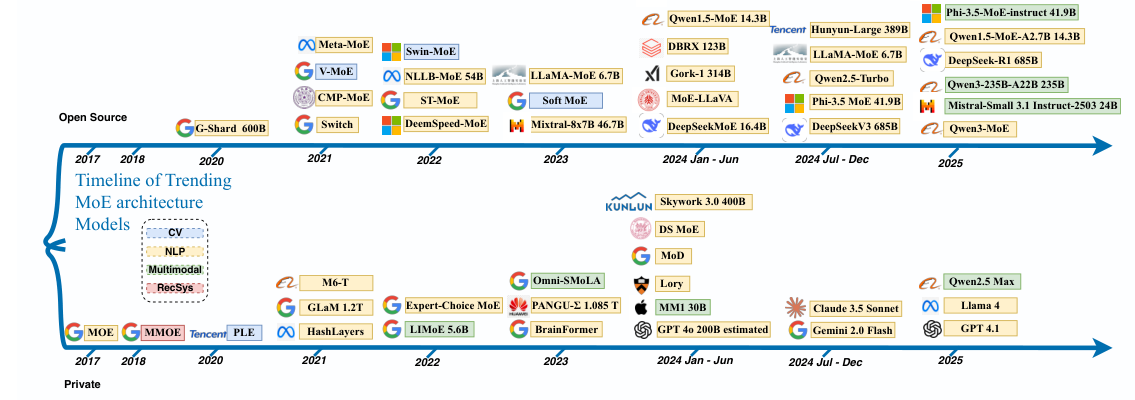
\includegraphics[width=\textwidth,height=0.82\textheight,keepaspectratio]{assets/New-Lecture-Transformers/moe_survey_fig1_timeline.png}
  \vspace{0.2em}
  {\scriptsize \textit{Reference:} Zhang et al., ``Mixture of Experts in Large Language Models,'' \href{https://arxiv.org/abs/2507.11181}{arXiv:2507.11181}.}
\end{frame}

\begin{frame}[t]{MoE for a decoder-only Transformer}
  \centering
  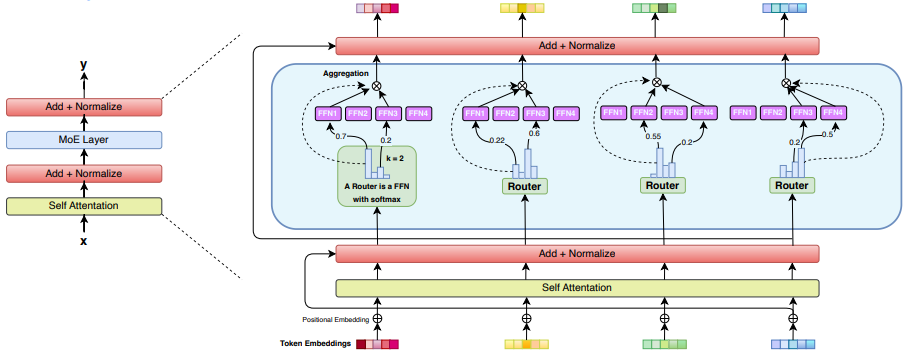
\includegraphics[width=\linewidth,height=0.62\textheight,keepaspectratio]{assets/New-Lecture-Transformers/moe_survey_fig5a_moe_layer.png}
  {\scriptsize MoE for a decoder-only Transformer with $k=2$ experts.}
  \begin{itemize}\footnotesize
    \item Input $\mathbf{x}$ enters a \textbf{gating / router} that outputs scores for each expert.
    \item Only the top-$k$ experts run their FFN; outputs are \textbf{combined} (often a weighted sum) for the residual stream.
  \end{itemize}
\end{frame}

% \begin{frame}[t]{Routing paradigms: token choice vs.\ expert choice}
%   \begin{itemize}
%     \item \textbf{Token choice (common in LLMs):} each token picks its favorite experts (e.g., top-2). Simple, but some experts can starve while others overload without load-balancing losses.
%     \item \textbf{Expert choice:} each expert receives a \textbf{fixed token budget} and selects which tokens it wants. Often improves utilization on structured or vision workloads.
%   \end{itemize}
% \end{frame}

\begin{frame}[t]{Example: Mixtral 8$\times$7B --- a common misconception}
  \begin{itemize}
    \item The name sounds like ``eight separate 7B models.'' The \textbf{released architecture is not that}: experts are \textbf{not} eight full standalone stacks.
    \item Instead, think ``\textbf{eight expert FFNs} per MoE layer, with \textbf{shared} attention and norms,'' and only a subset fires per token (here, \textbf{top-2} experts).
  \end{itemize}
  \centering
  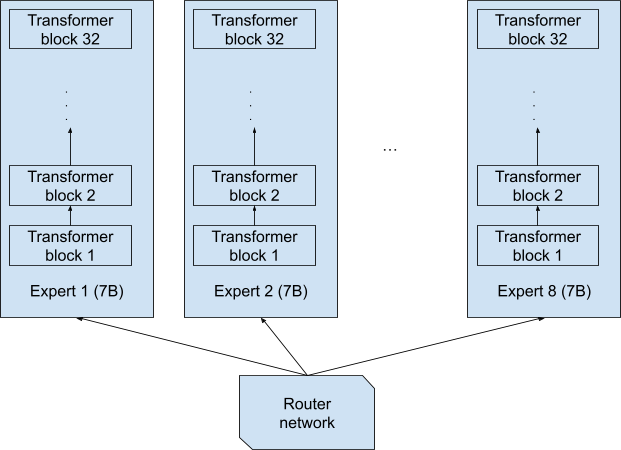
\includegraphics[width=0.72\textwidth,height=0.48\textheight,keepaspectratio]{assets/New-Lecture-Transformers/nvidia_blog_mixtral_misread_diagram.png}
  \vfill
  {\scriptsize \textit{Reference:} Kranen \& Nguyen, ``Applying Mixture of Experts in LLM Architectures,'' NVIDIA Technical Blog (2024), \href{https://developer.nvidia.com/blog/applying-mixture-of-experts-in-llm-architectures/}{article}.}
\end{frame}

\begin{frame}{MoE: Most Preferred Tokens By Experts}
  \centering
  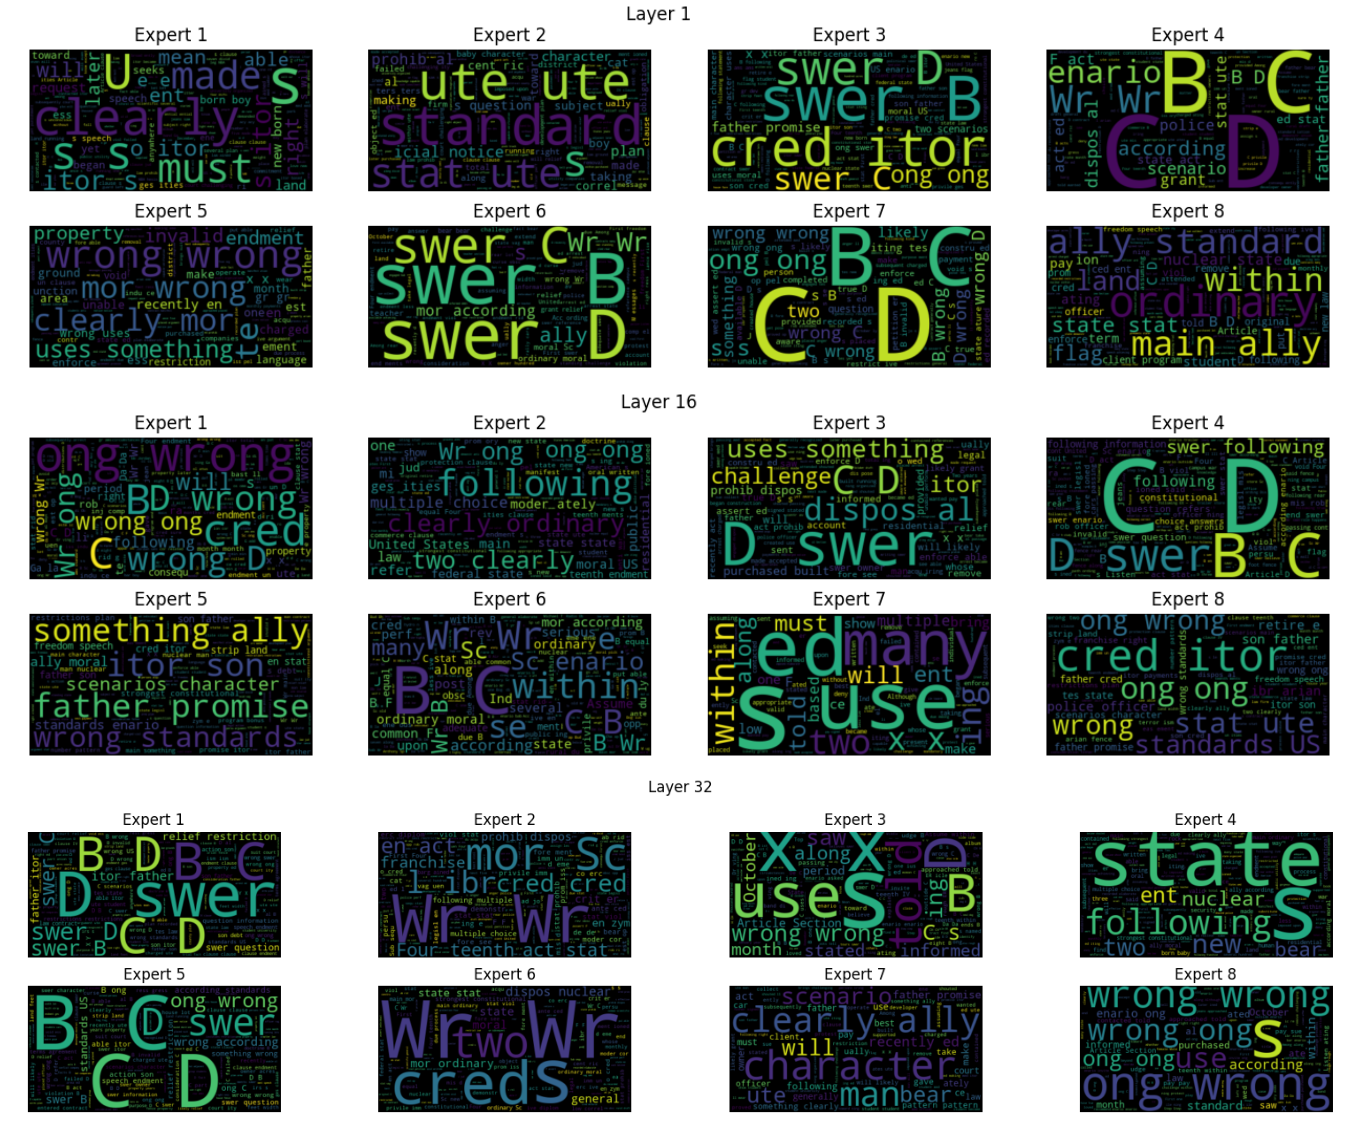
\includegraphics[width=\textwidth,height=0.78\textheight,keepaspectratio]{assets/New-Lecture-Transformers/most-common-tokens-processed-moe.png}
  \linebreak
  {\scriptsize \textit{Reference:} Kranen \& Nguyen, ``Applying Mixture of Experts in LLM Architectures,'' NVIDIA Technical Blog (2024), \href{https://developer.nvidia.com/blog/applying-mixture-of-experts-in-llm-architectures/}{article}.}
\end{frame}

% \begin{frame}[t]{MoE in production: what engineers worry about}
%   \begin{itemize}
%     \item \textbf{Load balancing:} auxiliary losses and schedule tricks so every expert sees enough tokens; otherwise routing collapses and capacity is wasted.
%     \item \textbf{All-to-all communication:} expert parallelism shuffles activations across GPUs---network and kernel design matter as much as math.
%     \item \textbf{Serving latency:} for large prompts where compute dominates, MoE can reduce \textbf{time-to-first-token}; for agentic / RAG loops, latency stacks across calls (blog motivation).
%     \item \textbf{Shared experts} (always on) plus routed experts appear in several frontier stacks to keep stable ``generalist'' capacity.
%   \end{itemize}
% \end{frame}
